\documentclass[10pt, french, a4paper]{report}

\usepackage[authoryear]{natbib}

\usepackage[textwidth=14cm]{geometry}
\usepackage{babel}
\usepackage{xcolor,graphicx}
\usepackage{hyperref}	
\usepackage{enumitem}
\usepackage{tabularx}
\usepackage{amsmath}


\renewcommand{\thechapter}{\Roman{chapter}}
\renewcommand{\contentsname}{Table des Matières}
\makeatletter
\renewcommand{\@chapapp}{Chapitre}
\makeatother

\setcounter{secnumdepth}{3}

\title{L'Ethique des Intelligences Artificielles :\newline Supervisation et confiance}
\author{Nathan Lauga}
\date{\today}

\begin{document}

% ======= PAGE TITRE ======== %

\begin{titlepage}
  \begin{center}

    
\includegraphics[height=1.3cm]{images/CEAPC_logo.png}
    \hspace{\fill}
    
\includegraphics[height=1.5cm]{images/ynov_informatique_logo.png}

    \vspace{2.5cm}
    {\scshape\LARGE Mémoire de Mastère\par}
    \vspace{1cm}
    {\scshape\Large Ynov Informatique Bordeaux\par}
    \vspace{0.5cm}
    {\scshape\large Mastère Data Science\par}
    \vspace{1cm}
    
    % Title
    \rule{\linewidth}{0.3mm} \\[0.4cm]
    { \huge \bfseries L'\uppercase{é}thique des Intelligences Artificielles \newline Supervisation et Confiance \\[0.4cm] }
    \rule{\linewidth}{0.3mm} \\[1cm]
  
    \vspace{1.5cm}

    \noindent
    \begin{minipage}{0.4\textwidth}
      \begin{flushleft} \large
        \textbf{Réalisé par :}\\
        M.~Nathan \textsc{Lauga}\\
      \end{flushleft}
    \end{minipage}%
    \begin{minipage}{0.5\textwidth}
      \begin{flushright} \large
        \textbf{Sous la direction de :} \\
        M.~Pascal \textsc{Fournier} [CEAPC]\\
        M.~Patrick \textsc{Piquart} [YNOV]\\
      \end{flushright}
    \end{minipage}\\[1cm]

    \vspace{2.5cm}

    {\scshape\Large 16 Août 2020\par}
    
  \end{center}
\end{titlepage}

\newpage
\setcounter{tocdepth}{3}
\tableofcontents

\newpage
\begin{abstract}

    Ceci est l'avant-propos.

\end{abstract}

% ====== INTRODUCTION ====== %

\newpage
\chapter*{Introduction}
\addcontentsline{toc}{chapter}{\protect\numberline{}Introduction}


% ======= ETAT DE L'ART ====== %
\chapter{\uppercase{é}tat de l'art}

\section{Les données et l'Intelligence Artificielle}

\begin{quotation}
  `` Si une machine peut penser, elle pourrait penser plus intelligemment que nous, et alors où devrions-nous être ? Si nous pouvions maintenir les machines dans une position servile, par exemple en coupant le courant à des moments stratégiques, nous devrions, en tant qu'espèce, nous sentir humbles. ''
\end{quotation}
\rightline{{\rm --- \citep{turing_browse_1951}}}

\paragraph{}
Le 15 mai 1951, Alan Turing, considéré comme le père de l'informatique, été interviewé par la BBC et annoncé déjà l'avènement probable des machines intelligentes, où plus particulièrement les machines pensentes. Bien qu'à cette époque nous étions loin des ordinateurs de nos jours, la force des propos de Turing montre que, dès la moitié du 20\textsuperscript{ème} siècle, le concept d'intelligence artificielle existait.

\paragraph{}
\underline{Intelligence artificielle :} En informatique, la recherche sur l'intelligence artificielle ou IA, est définie comme l'étude des ``agnets intelligents'', soit n'importe quel appareil qui perçoit son environnement et prend des déisions qui maximisent ses chances d'atteindre son objectif \citep{poole_computational_1997}. e.g. Dans les jeux d’échecs, un agent intelligent pourra, en connaissant les règles du jeu, effectuer des coups et son objectif, sera de battre son adversaire.

\subsection{La préface : Test de Turing, Systèmes Experts et les Hivers}

\begin{itemize}
  \item \underline{Algorithme :}
\end{itemize}

\paragraph{}
Le terme qui aujourd’hui, est très évocateur, a été utilisé pour la première fois en 1956 par John McCarthy, lors de la conférence de Darthmouth, conférence qui est considérée comme l’acte de naissance de l’intelligence artificielle en tant que domaine de recherche autonome \citep{solomonoff_time_1985}. Avant cela, l'utilisation de cette notion existait déjà et l'un des premiers articles discutant de cela remonte à 1945 avant même la première explosion atomique \citep{bush_as_1945}. Dans cet article, nous pouvons y voir les concepts d'ordinateurs, d'Internet ou encore de reconnaissance vocale.

\paragraph{}
En 1948, Robert Wiener, professeur au Massachusetts Institue of Technology (MIT) théorise la Cybernétique dans son livre ``Cybernétique ou la communication contrôlée dans le domaine de l'animal et de la machine''. Il décrit une théorie entière de la commande et de la communication, aussi bien chez l'animal que dans la machine \citep{wiener_cybernetics;_1961}. La but essentiel de la cybernétique est de comprendre et de définir des processus ou fonctions avec pour objectif de réagir par rapport à une certaine action en entrée. Il s'agit là de la préface au domaine de recherche de l'Intelligence Artificielle qui émergera à la conférence de Darthmouth évoquée dans le paragraphe précédent.

\paragraph{}
Lors de l'année 1950, la théorie du domaine étant à ses débuts, un nouveau papier permettra une grande avancée, celui d'Alan Turing \citep{turing_i.computing_1950}. Intitulé ``COMPUTING MACHINERY AND INTELLIGENCE''\footnote{Traduction : Les Machines Informatiques et l'Intelligence.}, il soumettra une question inédites : ``Les machines peuvent-elles penser ?''. Cette interrogation est très contradictoire, surtout en 1950, puisque le terme \textit{machine} et \textit{penser}, ne peuvent être définis d’une façon qui puisse satisfaire tout le monde. Afin de résoudre le conflit de cette contradiction, Turing a proposé une solution, élégante, étant le fameux ``Test de Turing''. 

\paragraph{}
\underline{Test de Turing :} Si une machine peut tenir une discussion avec un humain (au travers d’une messagerie par exemple), sans que la femme ou l’homme ne puisse distinguer qu’il s’agisse d’un humain ou d’une machine alors la définition du test dira que cette machine est "pensante". Il s’agit d’une proposition très importante dans la philosophie de l’intelligence artificielle \citep{pinar_saygin_turing_2000}. 

\paragraph{}
Les années suivants ces papiers, des déclarations comme ``d’ici dix ans un ordinateur sera le champion du monde des échecs'' \citep{simon_heuristic_1958} ou encore ``des machines seront capables, d’ici vingt ans, de faire tout travail que l’homme peut faire'' \citep{simon_shape_1965} crééront un engouement populaire dans le domaine de la recherche de l'Intelligence Artificielle. Ne s'agissant pas des seules déclarations à ce sujet, et celles-ci mènent à une attente très élevée concernant les possibilités des algorithmes intelligents, mais comme souvent lorsque les attentes sont élevées une phase de déception s’ensuit.

\paragraph{}
Dans les années 1970, apparu le premier hiver de l’histoire de l’intelligence artificielle. Comme une bulle qui aurait éclaté, la recherche a ralenti d’un coup, ainsi que le budget consacré au domaine. Les causes en sont multiples. Il est possible de retrouver entre autres, la limite de la puissance de calcul des ordinateurs ou encore le manque de base de connaissances du monde par les ordinateurs (manque de données). En effet, les travaux, qui portaient sur le langage naturel, ne pouvaient pas être extrêmement poussés puisque le stockage de la mémoire la limitait à vingt mots \citep{crevier_ai:_1992}. Pour beaucoup ce secteur a été enterré, mais arrivèrent les systèmes experts, programmes qui allient algorithme et connaissance métier. Ce concept qui comme le Soleil au printemps fit fondre la neige du premier hiver.

\paragraph{}
\underline{Système Expert :} c'est un programme capable de reproduire des patterns afin d'obtenir une sortie. Concrètement, c'est un logiciel qui avec une base de connaissances et une base de règle peut obtenir une réponse \citep{jackson_introduction_1998}. E.g. Un système expert peut avoir comme connaissance les polygones et leur nombre de côtés puis pour règle l'association comme trois côtés égal un triangle.

\paragraph{}
L’histoire se répéta malheureusement dans les années 90 : trop d’attente pour une réalité en dessous de l’imaginaire. La conséquence fut une nouvelle période froide dans ce domaine et un désenchantement populaire.

\begin{center}
  \begin{figure}[hbt!]
      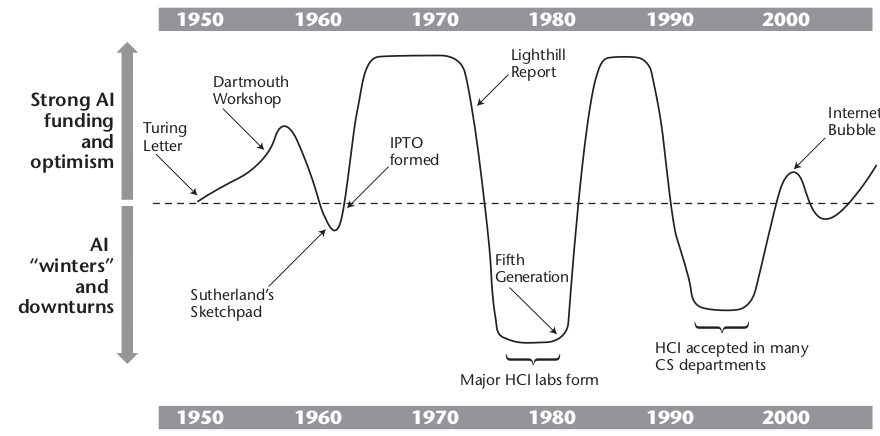
\includegraphics[width=\textwidth]{images/grudin_2009_changing_seasons_ai.png}
      \caption{Les saisons changeantes de l'IA \citep{grudin_ai_2009}}
  \end{figure}
\end{center}

\paragraph{}
Ci-dessus un résumé des débuts de l’histoire de l’intelligence artificielle avec en abscisse les années et en ordonnées l’attente autour de ce secteur. Sur le graphique, certains évènements majeurs de l’histoire du domaine en question. Aujourd'hui, grâce à plusieurs éléments l'IA retrouve une place dominante, entre autres la quantité de données à disposition a permi de faire exploser ce domaine de recherche. 

\subsection{Le changement des échelles de grandeurs : les données et Big Data}

\begin{quotation}
  ``Les données sont le nouveau pétrole. Il est précieux, mais s'il n'est pas raffiné, il ne peut pas vraiment être utilisé. Il doit être transformé en gaz, en plastique, en produits chimiques, etc. pour créer une entité de valeur qui stimule une activité rentable ; les données doivent donc être ventilées, analysées pour qu'elles aient de la valeur.''
\end{quotation}
\rightline{{\rm --- \citep{haupt_who_2006}}}

\paragraph{}
\underline{Données :} informations, notamment des faits ou chiffres, récoltées pour être étudiées et modifiées afin de faciliter une prise de décision. Les informations numériques sont stockées et exploitées par un ordinateur \citep{cambridge_data_2020}.

\paragraph{}
La compréhension de l'Intelligence Artificielle aujourd'hui, passe par obligatoirement par les données. En effet, les données sont le carburant, le nouveau pétrole\footnote{Cette métaphore a été utilisée par un grand nombre d'experts, mais le crédit de la première citation serait à attribuer à Clive Humby \citep{haupt_who_2006}.} L'analogie, bien que pertinente, a une limite : le pétrole est non-renouvelable, les données n'arrêtent pas d'augmenter.

\paragraph{}
L'augmentation de la quantité de données est liée aux progrès dans les capacités des systèmes de stockage, des techniques pour collecter les données et l'analyse de ces dernières \citep{press_very_2013}. Nous avons assisté à une sorte de Big Bang des informations numérisées lors de ces dernières décénies. Cette explosion est à la fois économique avec plus de 9,8 Milliards de Dollars investis en 2018, représentant une augmentation d'environ 75\% par rapport à 2017 \citep{columbus_25_2019}. Mais aussi en terme de volume : l'augmentation est telle que comme pour la loi de Moore\footnote{En somme, la loi de Moore consiste à dire que la complexité des microprocesseurs double pour une période de temps donnée \citep{moore_cramming_1998}.} la croissance de la quantité de données suit une courbe exponentielle. En effet, en 2018 la ``datasphère'' mondiale recensait environ 33 zettabytes\footnote{1 zettabyte vaut un billion de terabytes.} et selon IDC (International Data Council), en 2025, il y en aura 175 \citep{reinsel_digitization_2018}.

\begin{figure}[hbt!]
  \centering
  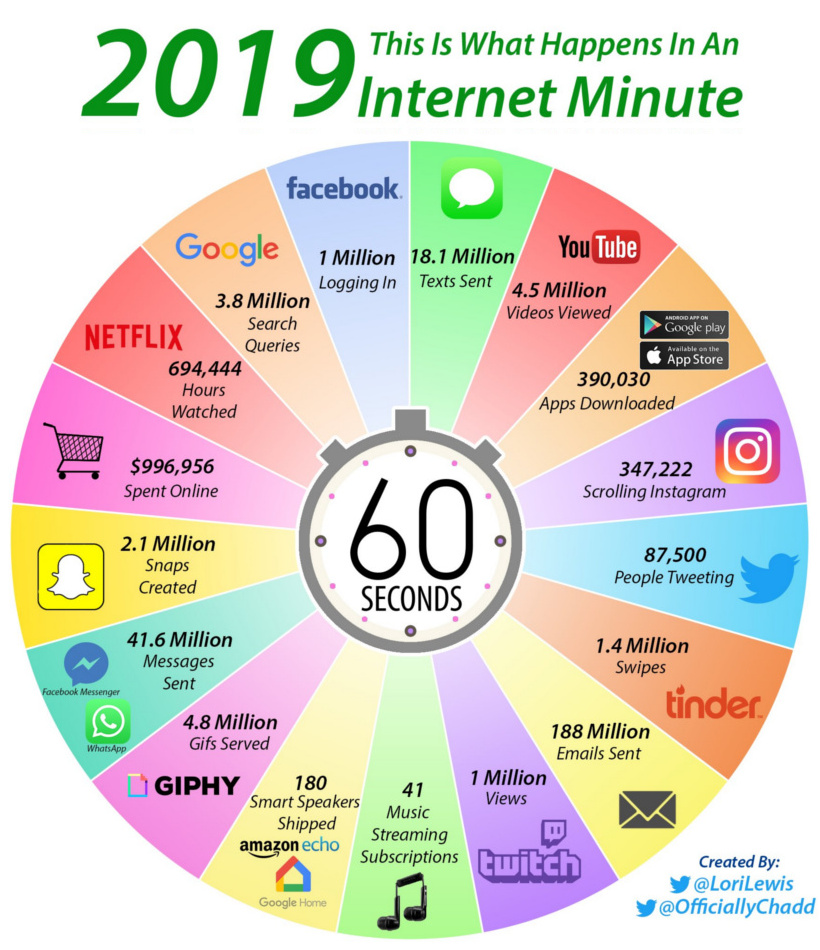
\includegraphics[width=0.4\textwidth]{images/internet-minute-2019.jpg}
  \caption{Ce qu'il se passe sur Internet en une minute en 2019 \citep{desjardins_what_2019}}
  \label{fig:internet_minute_2019}
\end{figure}

\paragraph{}
Cette immense collection de bits\footnote{Unité de stockage à la base de chaque ordinateur, peut uniquement prendre la valeur 0 ou 1.} est accentuée grâce aux fournisseurs que sont les utilisateurs massifs des grandes plateformes du web. En 2019, chaque minute c'est plus de 188 millions d'emails qui sont envoyés, environ 700 000 heures de vidéo Netflix regardées ou un million d'utilisateurs qui se connectent sur Facebook (voir figure \ref{fig:internet_minute_2019}).


\paragraph{}
Ce volume conséquent de données correspond au nouveau carburant des intelligences artificielles modernes. Les algorithmes utilisés dans ce domaine sont issus de la famille de l'apprentissage de la machine (où ``Machine Learning'' en anglais).

\subsection{L'Apprentissage de la Machine}

\paragraph{}
\underline{Modèle statistiques :} blabla

\subsubsection{L'Apprentissage Supervisé et Non Supervisé}

\paragraph{}

\subsubsection{Le processus de création d'une IA}

\paragraph{}

\subsection{Fiction ou Réalité : l'Intelligence Artificielle plus forte que les Humains}

\paragraph{}

\subsubsection{L'avènement de l'Intellect des Machines : Deep Learning}

\paragraph{}

\subsubsection{Les Intelligences Artificielles de demain : la singularité}

\paragraph{}

% ======= ETHIQUE ======== % 

\section{L'\uppercase{é}thique, la science de la Morale}

\subsection{L'origine du Bon, Histoire et Philosophie : Nietzsche}

\subsection{Philosophie, l'\uppercase{é}thique Normative}

% https://fr.wikipedia.org/wiki/%C3%89thique_normative

\subsubsection{Aristote et l'\uppercase{é}thique de la vertu}

% https://fr.wikipedia.org/wiki/%C3%89thique_de_la_vertu

\subsubsection{La Morale Déontologique : Kant et le mensonge}

\subsubsection{Le Conséquentialisme}

\subsection{La Morale en Science}

\subsubsection{L'Approche par la Culture et la Personnalité : le Culturalisme}

\subsubsection{Le cerveau précablé pour la Morale : l'hypothèse Naturaliste}
%http://homofabulus.com/sommes-nous-pre-cables-pour-etre-moraux-morale-2/
%https://fr.wikipedia.org/wiki/Naturalisme_moral


% ======= IA ET ETHIQUE ======== % 

\section{La question de l'\uppercase{é}thique pour les algorithmes intelligents}

\subsection{La recherche du domaine : une IA de confiance selon la Commission Européenne}

\subsubsection{Les lois pour contrôler : Justice et Licité}

\subsubsection{L'\uppercase{é}thique hypothétique d'une IA Morale}

\subsubsection{Sécurité et la Robustesse Technique}

\subsection{Les problèmes du Présent}

\subsubsection{La Discrimiation des algorithmes : les biais}

\subsubsection{Ouvrir la boîte noire : Interprétabilité et Explicabilité}

\subsubsection{Les créateurs des IA, architectes de notre quotidien}

\subsection{Les Dilemmes Moraux pour les Machines}

\subsubsection{Expliciter la morale des humains}

\subsubsection{La décision par l'Aléatoire : Alexei Grinbaum}

\section{Synthèse}

% ======= SOLUTION ===== %
\newpage
\chapter{Solution : une boîte à outils transparente}

\section{Travaux connexes}

\subsection{La détection et atténuation des biais}

\subsubsection{Mesure des biais : calculer l'impact social}

\paragraph{Statistical Parity Difference}

\paragraph{Equal Opportunity Difference}

\paragraph{Average Odds Difference}

\paragraph{Disparact Impact}

\paragraph{Theil Index}

\paragraph{Définition de mesures ``morales'' sur les biais}

\subsubsection{AIF360 : AI Fairness 360 par IBM}

\paragraph{Fonctionnement technique}

\paragraph{Les algorithmes de mitigation des biais}

\subsection{L'explication des résultats d'une IA}

\subsubsection{LIME : Local Interpretable Model-agnostic Explanations}

\subsubsection{SHAP : SHapley Additive exPlanations}

\subsubsection{Ethik}

\subsection{Cadrage de l'IA}

\subsubsection{ML Canvas}

\subsubsection{PAIR Guidebook}

\section{TransparentAI : de la théorie à la pratique}

\subsection{Philosophie : Open-Source et compréhensible}

\subsubsection{Pourquoi créer cet outil ?}

\subsubsection{Structure de la boîte à outil}

\subsection{Répondre à la question "Est-ce que mon IA est responsable ?"}

\subsubsection{Les fonctionnalités}

\section{Synthèse}


% ======= PLAN DE RECHERCHE ===== %
\newpage
\chapter{Plan de recherche}

% ====== CONCLUSION ====== %

\newpage
\chapter*{Conclusion}
\addcontentsline{toc}{chapter}{\protect\numberline{}Conclusion}

\newpage
% \bibliographystyle{alpha}
\bibliographystyle{plainnat}
\bibliography{bibliography}

\end{document}